\index{Seismic Sources!Model}
\index{Seismic Sources!Initial Model}
The Earthquake Rupture Forecast is a fundamental concept in the OpenSHA framework and, accordingly, within the hazard component of OpenQuake.

%
The calculation of the Seismicity Occurrence Model (that is the Earthquake Rupture Forecast) starts from a Seismic Sources model i.e. a complete description of the type, geometry and seismicity occurrence properties of each seismic source necessary to calculate the hazard over the investigated area. A Seismic Sources Model doesn't incorporate any epistemic uncertainties, since it represents the crudest and simplest description of the information necessary to compute PSHA.

%
According to the previous chapter, OpenQuake prepares a Seismic Sources Model (SSM) by provinding with a calculator - named Logic Tree Processor (LTP) - the Initial Seismic Sources Models and the Seismic Sources Logic Tree (the ensamble of these objects is called the Seismic Sources System).

%
The OQ Earthquake Rupture Forecast calculator takes the SSM and creates a list of the ruptures generated by all the sources incorporated in the SSM. Each rupture in the Earthquake Rupture Focast is associated with a probability of occurrence in the time span specified in the calculation settings. 
Is worth to mention that: 
\begin{itemize}
\item every source typology in the Seismic Sources Model has a customised treatment in the Earthquake Rupture Forecast calculator;
\item for the time being, we support only sources generating seismicity in time accoording to a Possion temporal occurrence model.
\end{itemize}

%
In the following paragraphs we describe the way OpenQuake creates the ERF using the  seismic source typologies currently supported, in agreement with the input specifications described in Chapter \ref{chap:hazinp}.
%
% ------------------------------------------------------------------------------
\section{ERF creation in case of distributed seismicity}
Open Quake supports two seismic source typologies capable to model distributed seismicity: area sources and grid sources.

Area sources are the most traditional source type adopted in PSHA analysis since 
its first introduction at the end of the 1960s. On the contracry, grid sources were more recently adopted in hazard calculation. The works of \cite{frankel1995} and \cite{frankel1997} boosted their use in probabilistic seismic hazard calculations. 
%
%  - - - - - - - - - - - - - - - - - - - - - - - - - - - - - - - - - - - - - - -
\subsection{Area sources}
%
The creation of an ERF in case of area sources (see also Section \ref{hazard:seismic_source_types:areaSources} at page \pageref{hazard:seismic_source_types:areaSources}) requires a preliminary step 
consisting in the discretization of the polygon used to delimit the spatial extension of the source. 

%
% . . . . . . . . . . . . . . . . . . . . . . . . . . . . . . . . . . . > Figure
\begin{figure}[!ht]
\centering
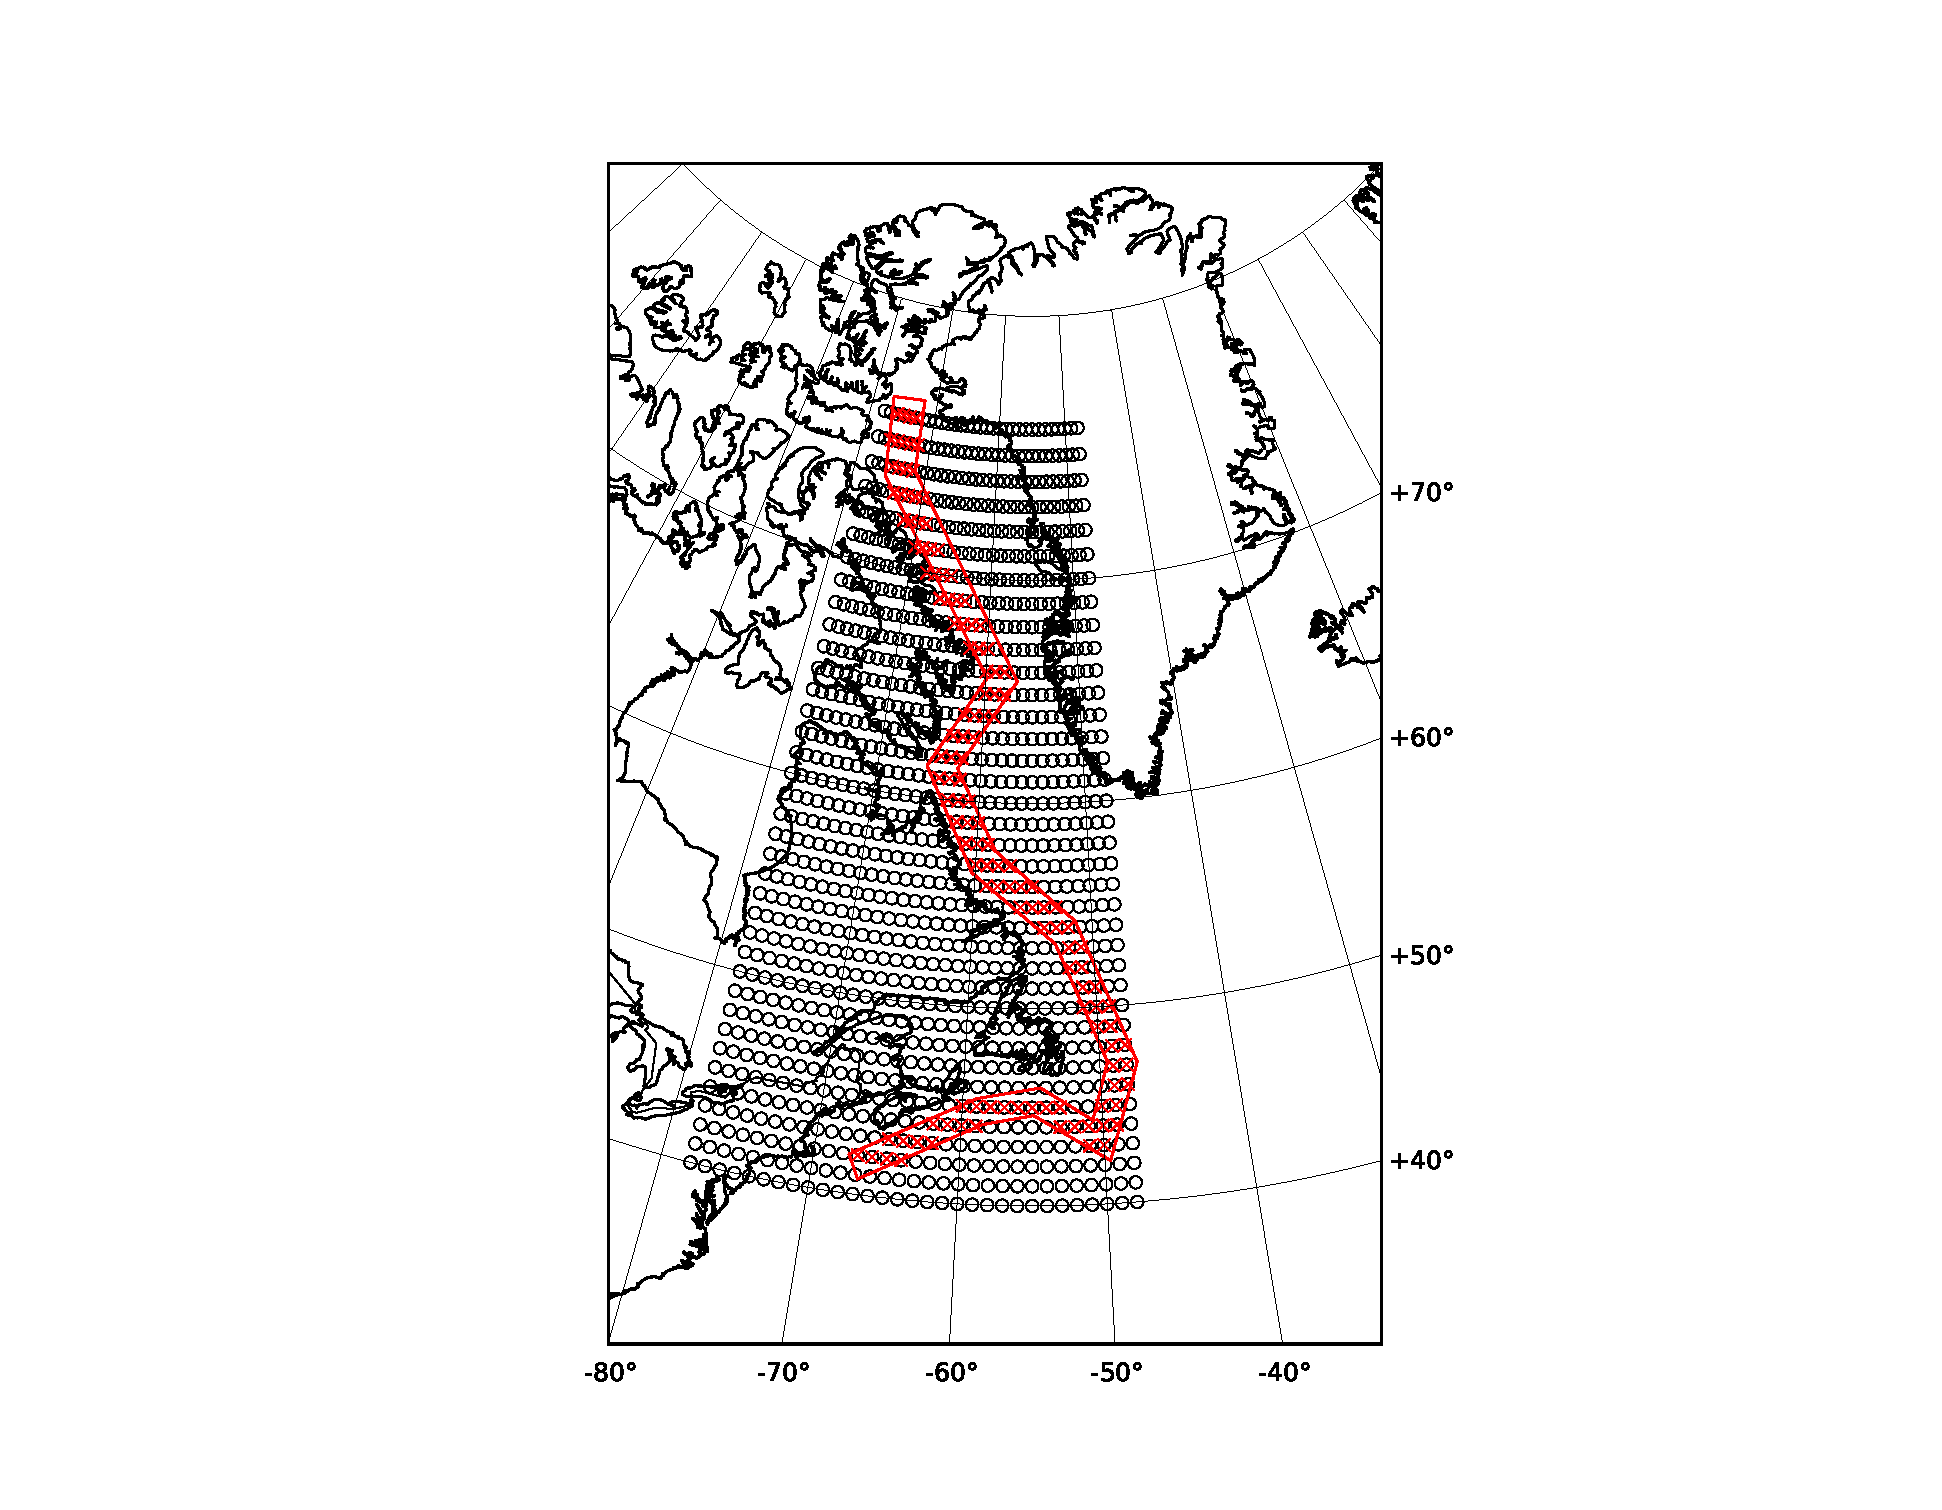
\includegraphics[width=18cm]{./Figures/Part_Hazard/area_source_discretization.eps}
\caption{Example of an area source discretisation (grid spacing equal to 0.5$^\circ$).}
\label{fig:area_source_discret}
\end{figure}
% . . . . . . . . . . . . . . . . . . . . . . . . . . . . . . . . . . . < Figure
%

OQ discretizes area sources by overlapping over the polygon a regular grid of nodes. OQ uses the nodes inside the polygon to represent - in a discrete way - the area source.
The grid contains nodes equally spaced in latitude and longitude; the position of each node is specified by one geographic coordinate, expressed in decimal degrees. 
%
Exidently, this grid structure implies that the spacing in longitude between nodes is dependent on the latitude. The spacing of two nearby nodes near the equator is larger than at high latitudes. E.g. one degree of longitude at the equator correponds to about 111 km, at 45$^\circ$ of latitude it becomes about 78.8 km and, at 75$^\circ$ it corresponds to only 28 km. 
 
Figure \ref{fig:area_source_discret} shows a discretization example considering an area source contained in the Canada model. 
%
To guarantee an homogeneous distribution of seismicity rates OQ scales the seismicity proportionally to the cell size. For each cell of each area source we compute the area using the following (simplified) relationship:
\begin{equation}
 \text{cell\_area} = 4\pi^2 * \text{grid\_spacing}^2 *  
 	\left(\frac{\text{earth\_radius}}{360}\right)^2 * 
 	\sin(\text{cell\_latitude})
\end{equation}
where:
\begin{itemize}
\item grid\_spacing is the distance between two consecutive cells of the grid  
	adopted to discretize the area source 
\item earth\_radius is the mean radius of the Earth (approximately 6371 km) 
\item cell\_latitude is the latitude of the cell of which we compute the area.
\end{itemize}
%
The weight for cell $w_n$ in a given area source is equal to the ratio between the area of the source (i.e. the sum of the areas of the cells included) and the 
area of the cell.
% 
OQ computes the frequency-magnitude distribution for cell $n$ by multiplying the 
FMD defined for the entire area source by the corresponding weight $w_n$. 

\textcolor{red}{CONTROLLARE}\dotfill \\
In the simplest case where the user do not specify any faulting style The seismicity - specified in the input file in terms of discrete frequency-magnitude distribution i.e. a set of tuples $<M=m,\lambda_m>$ each one specifying an occurrence rate w.r.t. a magnitude value 

%
%  - - - - - - - - - - - - - - - - - - - - - - - - - - - - - - - - - - - - - - -
\subsection{Multi-depth Area sources}
%
This source typology is basically an extension of the simpler area source since 
it allows to distribute seismicity with depth.

%
%  - - - - - - - - - - - - - - - - - - - - - - - - - - - - - - - - - - - - - - -
\subsection{Grid sources}
The creation of the ERF in case of grid sources follows the same concepts described in the previous section in case of area sources. The main difference is that with this source type the discretisation step is not needed.

%  - - - - - - - - - - - - - - - - - - - - - - - - - - - - - - - - - - - - - - -
\subsection{Accounting for rupture finiteness in case of distributed seismicity}
%
Each node $x$ used to discretise an area source or belonging to a grid source  has $fm_{x}$ tuples composed by the following objects:
\begin{itemize}
\item A discrete representation of a Frequency-Magnitude Distribution (FMD);
\item A faulting style, that is strike [optional], dip [optional] and rake [optional] 
\end{itemize}
The definition of one, or several, faulting styles is optional; this means that 
in the simplest case only one discrete FMD is specified.
Depending on the parameters specified in the faulting style, OQ takes the following actions:
\begin{enumerate}
\item No faulting style parameters specified:
	\begin{enumerate}
	\item In case finite ruptures requested for the Grid Seismic Source under consideration, OQ generates finite ruptures 
	\end{enumerate}
\item Only strike specified:
	\begin{enumerate}
	\item In case finite ruptures requested for the Grid Seismic Source under consideration, OQ generates finite rupt
	\end{enumerate}
\item
\end{enumerate}

%
% ------------------------------------------------------------------------------
\section{ERF creation in case of Fault sources}

%
%  . . . . . . . . . . . . . . . . . . . . . . . . . . . . . . . . . . . . . . .
\subsection{Fault sources with simple geometry}
Simple faults in OQ are representations of tectonic structures with a . The methodology adopted fot the creation of the fault surface uses the fault trace, a representative dip direction (e.g. it could be the mean dip direction) and, the upper and lower seismogenic depth. 

%
%  . . . . . . . . . . . . . . . . . . . . . . . . . . . . . . . . . . . . . . .
\subsection{Fault sources with complex geometry}

%
% ------------------------------------------------------------------------------
\section{Computing the probability of occurrence of each rupture}
In OQ, by convention, we describe the frequency-magnitude distribution using a discrete representation. This choice offers the largest flexibility in describing the rate of earthquakes with respect to magnitude. 
%
% . . . . . . . . . . . . . . . . . . . . . . . . . . . . . . . . . . . > Figure
\begin{figure}[!ht]
\includegraphics[width=15cm]{./Figures/Part_Hazard/gr_example.eps}
\caption{Example of a discrete incremental frequency-magnitude Gutenberg-Richter distribution}
\label{fig:gr-example}
\end{figure}
% . . . . . . . . . . . . . . . . . . . . . . . . . . . . . . . . . . . < Figure
%

